\section{Episode 55: Breakfast Cat - Origins}

\textbf{4 YEARS EARLIER - SOMEWHERE IN VELTERRA} \medskip

A jungle, a chase. Small green feet, running. Something crashing through the undergrowth. A small goblin girl pants, trying to glance over her shoulder, tripping slightly as she does so. She picks herself up off the ground, just as the bushes get torn apart and a medium-sized giant boar bellows at her, spit flying from its maw.\medskip

“KOLLLLOOOOOOOOOOOOOO!”\medskip

She hears no response, and the boar advances upon her prone, panicked form. She feels the hot, wet air against her face, and closes her eyes. She opens them, just to see a stone impact the side of the pig’s head, sending it crashing to the ground. “Hahahhaarrghh, silly piggy”. “Oh, Kolo, I thought I was going to die, I thought I was alone". “Don’t worry Exme, you’ll never be alone”. \medskip

Dissolve to Exme’s face, covered in blood.\medskip

Exme, backed by a mournful acoustic cover, begins the long and gruesome process of cleaning up after the night before. There’s a montage. She goes to sleep on the top deck, the stone of Unthala clutched to her chest. When she wakes up in literal hell, rather than her personal hell, [that elephant lady] brings her into Lazarus’s office. Lazarus is sat scribbling furiously at his desk. Exme, with steely determination, sits in the desk, waiting for him to finish. She doesn’t give Lazarus any choice. He must help. He doesn’t.\medskip

He knows the direction Kolo went, and that he can’t be reached via the stone any more. Exme is unimpressed. She asks why Lazarus hasn’t helped before now, and he asks a similar question back, pointing out that it was quite apparent that something was wrong with Kolo. He has done everything he can. Exme, getting nowhere with Laz, promises him that if she doesn't get what she wants, she will burn down the the whole of hell. She leaves, and wakes up several hours later to the smell of cooking eggs. Lillith shouts up from below deck, trying to wake everyone up with the promise of delicious breakfast.\medskip

Burnie and Delilah find Exme and ask her what’s wrong. Exme tells them everything, but that it will be okay, because they’ll sort it out. They go downstairs. Kolo has smashed up a lot of his lab, but the ingredients for the destoning potion are on the side, along with the instructions. Exme thinks she'll be able to reproduce them, given time. Lillith, doing her bit, has placed humorous hats upon Myron and Rip, to lighten the mood slightly. As they are having breakfast, Delilah reports that there is a stagecoach, of Hope’s Restian design, parked underneath the airship.\medskip

Lillith and Burnie head down to greet the guest, discussing tactics on the way. They’ll do the old one-two, where only one person talks, despite there being two people. They approach the carriage, and out steps a large, well dressed tiger carrying a briefcase, and holding a cane he clearly doesn't need. He steps down and asks them if they are associated of Riphard Obsidian Hardstone. Lillith says no, and Burnie says yes, and for some reason, the tiger believes Burnie. The tiger informs them that he is from the Guilds of Coin and his here in regards to Riphard’s fortune. Lillith introduces herself as Burnie’s solicitor, Burnie as Riphard’s sole heir with “whatever name he makes up”, and Riphard as turned into stone forever. It is unclear, even to Lillith, what the purpose of this deception is.\medskip

[Reports including a section of proceedings have been lost in the flooding of a record's office in the Age of Abject Terrors, a section of the correspondences between Anthony Tigerius and the Guild of Coin have been donated by the Tigerius Estate, to cover a section of this missing period]\medskip

-- Letters to The Guild of Coin Issue 0.5 -- :Fragment:\medskip
\textit{
Good news for once,

I have finally tracked down the elusive groups airship, instead of an object of high fantasy it is very much real and does indeed possess the ability to just float in the sky. Sky ships such as this could revolutionise travel across the planet, a new investigation should be opened into them alone. For now I have a more pressing matter to attend to. Riphard compatriots seem intent on lying about everything, although after a time it is possible to see the grains of truth among the nonsense.

There is always a cloud within the silver lining, and it seems that Riphard is currently made entirely of stone. How this transpired I find hard to swallow, but either way he seems currently ill disposed for our required discussions. Instead I find he has a partner who carries his heir, she is amenable and as per protocol I offer her the full services of the guild.

A small goblin seems convinced that she can bring Riphard back, either way I have finally found the owner/s of the bank and shall proceed...

The group seem set on finding something they are calling Excalibrum, they offer little to no explanation as to why, but seem to buy that I would be keen to join them so that I may see the sights of the ancient dwarven ruins, from which they rose to fantastical riches. Having only just found them, I am loathe to let them out of my sight. If the tales were true about the airship, then perhaps this group really is as capable and insane as they say.

The city is still in turmoil, and it seems to be from no small part of this party. Details are sketchy, and the group are still set on flagrant lies rather than comprehensive answers. However we put that aside, I am sure the destabilisation of one of the richest cities the planet has ever known will offer more opportunity for investment and growth than its closed doors had previously.

We enter the mines, and I am struck by the great efforts the Dwarves must have gone through to establish such a system. In a bid to expedite our arrival at an unknown location within the bowls of the mines, the goblin sets up a giant mechanised bear for us to ride down the mine cart rails. Good grief, I can see why it was hard to swallow our other reports.

The deeper we go the more elaborate the architecture becomes, it seems like the depths were more ostentatious than the heights. We pass countless ruins of past dwarven civilisation before arriving at a rune scrubbed arch way a full 2 days after we set off.

[Content Missing]
}\medskip

After checking that the second tomb isn’t trapped, Lillith decides to get someone with more upper body strength to open it, anyway. Burnie reaches completes his experience with the statue, and rejoins the group, looking flushed. Lillith immediately gets Burnie to open the tomb for her, and he immediately spots the trap. He dodges out the way, but there is nothing interesting inside apart from a snazzy necklace, which he puts on while he opens the other tombs, which are also boringly empty. After admiring the engravings for a bit, they leave the room and head up to the other corridor, where the detectomatic detected a bit of magic. Burnie picks the lock and goes through the grated door that blocks the upper corridor, it reveals a large crystaline orb, glowing a soft milky white. Anthony pads down, and pokes his head round an open door that leads off to the right. He sees some paw prints, that look like something dog-sized but not dog-variety, but nothing else.\medskip

The orb seems to be half a broken communication system, and not of any particular interest right now, so they go back and try another door leading out the of the room with the statue in it. Stairs lead up, to a room with an empty casket for no reason. Burnie starts daydreaming about vampire erotica, Anthony trots off, excitedly poking through a web-covered hallway, into a large web-covered room. Burnie starts burning the webs away, when two giant blue and white spiders appear out of nowhere and begin attacking the party. Anthony shoots it with a bow, and then Exme makes her look foolish by eviscerating one with her gun. Lillith doesn’t even know that anything’s the matter. Stanri bites the other one, it bites back, and then promptly disappears.\medskip

For some spurious reason, they don’t assume that this solves their problem, and they all wait to see if something interesting happens. Lillith moves through the webs, which are icky. While her back is turned, the spider reappears and everyone kills it. They jauntily carry on down the corridor. They arrive at a junction, and decide to head on down the most obviously trapped corridor. The obviously trapped corridor turns out to secretly be not trapped, but does contain a gross cloaker, which flies at Burnie and then everyone attacks it, it makes a weird noise, and then dies too. They carry on, and arrive in another space where the ground has fallen partly away, leaving platforms standing isolated a few dozen feet above jagged rocks. Stanri forms a bridge, and everyone strolls across. They pass a turning off to the left, but Anthony fires a grappling hook off to carry straight on, spuriously.\medskip

The gang leave Stanri behind as they go onwards past a statue which Anthony seems to think is of the god Aladoon, but the bookburners assure him is a statue of a particularly Good Dog, and it must be true because they read it in a really badly spelled book. Anthony carries on, and finds a room with a big pit in it. He looks down into it, and sees a red, horned face looking at at him, as a four armed, horned abomination climbs out of the hole. It throws him backwards, and emanates a dark, thick blackness which fills the room, covering Anthony and Burnie. Lillith drags Esme backwards out of the darkness, says there’s nothing to be done, and makes her way towards the exit. Exme is unimpressed.\medskip

The thing crushes Burnie in a giant lobster claw, and continues to just be generally awful. Exmie shoots blindly into the darkness, aiming roughly at where Burnie’s voice is shouting words of encouragement, blasting a large hole into the creature, which drops the darkness, so that it can cause Anthony and Burnie to become confused. Exme and Stanri both try and coerce Lillith to enter the fray, but she refuses to do any more than poke her head round the corner and fail to do anything useful with her crossbow, before running off and hiding round the corner. [Someone] gets enough of a hit on the thing that it is unable to hold its befuddling effect on the minds of Burnie and Anthony. Instead, it focuses its attention on Burnie, held bleeding in its claw, and Burnie becomes stunned, fixated on the sheer awfulness of the situation.\medskip

Refusing to be drawn into charging into battle by Stanri or Exme, Lillith cautiously pokes her head round the corner to see Burnie hanging helpless and stunned in the claws of something that should definitely not exist. She sighs, overcomes her self-preservation instincts, charges into battle, slides underneath Burnie and attempts to pull him from the claw by the ankles. She completely fails. As the last of Burnie’s ribs crack within the chitinous claw of the beast, Anthony gets peeved about the injustice of it all. He gets real peeved. In his peeved state, he bites his lip and spits blood as he expresses his displeasure at the current situation. His consternation taps into a primal fury, and the mild-mannered Anthony gives way to a blur of cane-sword and rage, pounding against the exterior surface of the not-a-demon. Life flickers momentarily into Burnie as he is lifted into the air, for the finishing blow. As the monster brings him back down, Burnie has shifted his sword, Wasabi, into position, and it plunges into the belly of the beast.\medskip

Burnie and the horned beast both collapse to the ground as Anthony runs off, blood still pouring out his mouth. Lillith tells Burnie that she’s only going to put herself on the line for him once, and that was it. He reminds her that she did it really badly. Exme runs off to check on Anthony. Anthony is trying desperately to murder a dwarf that’s been dead for hundreds of years, in a small crypt just off the previous area. Once he’s calmed down slightly, he apologises to Exme for acting so uncouthly. Everyone else joins them in the crypt as Exme pays close attention to a statue of Synn in the corner, and Anthony fails to force open a chest. Exme says that they shouldn’t open it, because this guy was seemingly blessed by Synn, and they have that in common, but no one can hear her over the sound of Lillith opening the chest. Inside they find a shit tonne of gems, an old book, and a dagger.\medskip

Exme works out that the book is a manual of RuneCarving and the dagger is covered in awesome runes that make it great. Everyone is interested, but very tired. They decide that they should probably rest in this crypt for a bit, before heading out to get the metal in the morning. \medskip

https://www.youtube.com/watch?v=RFyCPicGbXM\medskip

\textbf{Epilogue}\medskip

In the dark of the crypt, the only light is the dim green light illuminating the face of the goblin woman as she types feverishly using a keyboard built into the side of her bear. Green text flicks across the screen as a bar moves slowly across the horizontal axis of the display.\medskip

She pauses as the bar reaches the right hand side, and moves the processed data to a folder marked “Locashun Scans” and into a subfolder titled “Lazzyrus’s Place”, before selecting the file and pressing a very specific selection of buttons.\medskip

The images on the screen are replaced by flashing text repeating “Processing Battle Simulations”, “Analysing Weaknesses”, “Preparing Tactical Portfolio”, “ ; ) “ as she smiles contentedly, closing the hatch concealing the console, giving her bear a pat on the rump and settling down to sleep.\medskip

\vspace*{5mm}

\begin{center}
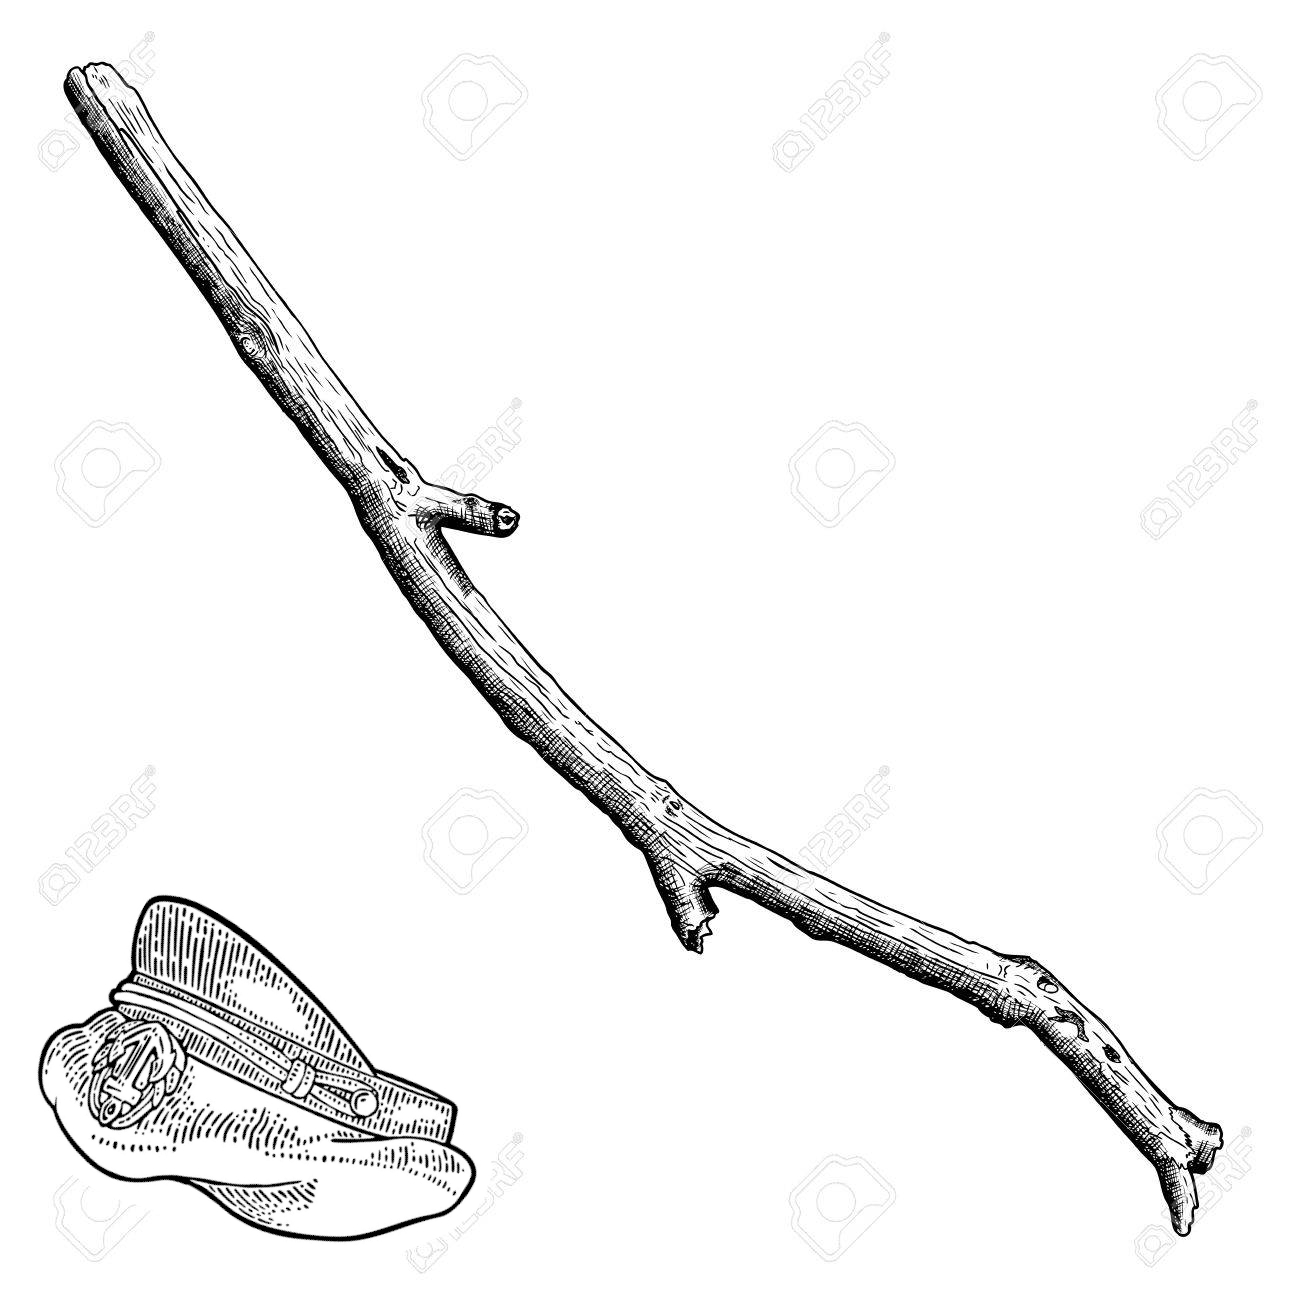
\includegraphics[width=\textwidth]{./content/img/xxx.jpg}
\begin{figure}[h]
\end{figure}
\end{center}

\clearpage